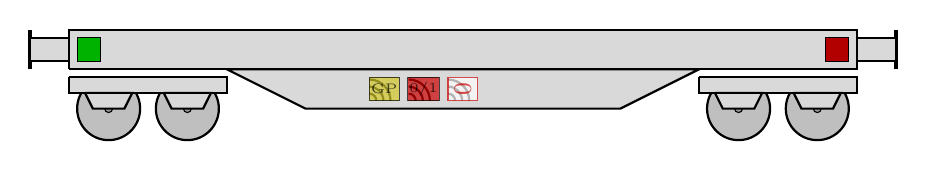
\begin{tikzpicture}[font = \sffamily]
%        \node (a) at (0,0) {};
%        \node (b) at (6,0) {};
        \draw[fill = gray!30, thick] (0,3) -- (10,3) -- (10,3.5) -- (0,3.5) -- (0,3);
        \draw[fill = gray!30, thick] (2,3) -- (3,2.5) -- (7,2.5) -- (8,3) -- (2,3);
        %DG 1
        \draw[fill = gray!50, thick] (8.5, 2.5) circle[radius = .4cm];
        \draw[fill = gray!80] (8.5, 2.5) circle[radius = .05cm];
        \draw[fill = gray!50, thick] (9.5, 2.5) circle[radius = .4cm];
        \draw[fill = gray!80] (9.5, 2.5) circle[radius = .05cm];
			\draw[fill = gray!30, thick] (8,2.9) -- (10,2.9) -- (10,2.7) -- (8,2.7) -- (8,2.9);
			\draw[fill = gray!30, thick] (8.2,2.7) -- (8.3,2.5) -- (8.7,2.5) -- (8.8,2.7) -- (8.2,2.7);
			\draw[fill = gray!30, thick] (9.2,2.7) -- (9.3,2.5) -- (9.7,2.5) -- (9.8,2.7) -- (9.2,2.7);
        %DG 2
        \draw[fill = gray!50, thick] (0.5, 2.5) circle[radius = .4cm];
        \draw[fill = gray!80] (0.5, 2.5) circle[radius = .05cm];
        \draw[fill = gray!50, thick] (1.5, 2.5) circle[radius = .4cm];
        \draw[fill = gray!80] (1.5, 2.5) circle[radius = .05cm];
			\draw[fill = gray!30, thick] (0,2.9) -- (2,2.9) -- (2,2.7) -- (0,2.7) -- (0,2.9);
			\draw[fill = gray!30, thick] (0.2,2.7) -- (0.3,2.5) -- (0.7,2.5) -- (0.8,2.7) -- (0.2,2.7);
			\draw[fill = gray!30, thick] (1.2,2.7) -- (1.3,2.5) -- (1.7,2.5) -- (1.8,2.7) -- (1.2,2.7);
	%Puffer 2
			\draw[ultra thick] (10.5,3) -- (10.5, 3.5);
			\draw[fill = gray!30, thick] (10.5,3.1) -- (10,3.1) -- (10,3.4) -- (10.5,3.4) -- (10.5,3.1);
	%Puffer 2
			\draw[ultra thick] (-.5,3) -- (-.5, 3.5);
	 		\draw[fill = gray!30, thick] (-.5,3.1) -- (0,3.1) -- (0,3.4) -- (-.5,3.4) -- (-.5,3.1);
			% Neues UIC-Zeichen
			%\node [cloud, cloud puffs=9, draw = none, fill = yellow!80!black, minimum width=.8cm, minimum height=.3cm, font = \tiny, inner sep = 0] at (4, 3.25) {4.0};
			% Aussenanzeigen
			\draw[fill = green!70!black] (0.1,3.1) -- (0.4,3.1) -- (0.4,3.4) -- (0.1,3.4) -- (0.1,3.1);
			\draw[fill = red!70!black] (9.9,3.1) -- (9.6,3.1) -- (9.6,3.4) -- (9.9,3.4) -- (9.9,3.1);
			%\node[draw, fill = white, font = \small, inner sep = 0.6, minimum height = 0.3cm] at (4, 3.25) {P 86};
			\draw[thick] (3.90, 2.6) arc (0:90:.09cm);
			\draw[thick] (3.99, 2.6) arc (0:90:.18cm);
			\draw[thick] (4.08, 2.6) arc (0:90:.27cm);
			\node[opacity = .7, draw, fill = yellow!80!black, font = \tiny, inner sep = 0.6, minimum height = 0.3cm, minimum width = 0.38cm] at (4, 2.75) {GP};
			\draw[thick] (4.40, 2.6) arc (0:90:.09cm);
			\draw[thick] (4.49, 2.6) arc (0:90:.18cm);
			\draw[thick] (4.58, 2.6) arc (0:90:.27cm);
			\node[opacity = 0.7, draw, fill = red!80!black, font = \tiny, inner sep = 0.6, minimum height = 0.3cm, minimum width = 0.38cm] at (4.5, 2.75) {0/1};
			\draw[thick] (4.90, 2.6) arc (0:90:.09cm);
			\draw[thick] (4.99, 2.6) arc (0:90:.18cm);
			\draw[thick] (5.08, 2.6) arc (0:90:.27cm);
			\node[opacity = 0.7, draw = red!80!black, text = red!80!black, fill = white, font = \small, inner sep = 0.6, minimum height = 0.38cm, minimum width = 0.3cm, rotate = 90] at (5, 2.75) {0};

\end{tikzpicture}
